\documentclass[thesis=B,czech]{FITthesis}[2012/06/26]

\usepackage[utf8]{inputenc}
\usepackage{pdfpages}
\usepackage{graphicx}
\usepackage{minted}
\usepackage{dirtree}

\definecolor{bgcode}{rgb}{0.95,0.95,0.95}
\definecolor{dangerred}{rgb}{0.91,0.13,0.16}

% % list of acronyms
% \usepackage[acronym,nonumberlist,toc,numberedsection=autolabel]{glossaries}
% \iflanguage{czech}{\renewcommand*{\acronymname}{Seznam pou{\v z}it{\' y}ch zkratek}}{}
% \makeglossaries

\renewcommand \listingscaption{Ukázka kódu}
\renewcommand \listoflistingscaption{Seznam ukázek kódu}

\newcommand{\inlinestr}[1]{\colorbox{bgcode}{\textit{#1}}}

\newcommand{\vapi}{1.2.15}

\newcommand{\todo}[1]{
	{\Large \color{dangerred} \textbf{TODO:} #1 \par}
}

% Shorcut for Swift code listings
\newcommand{\swiftcode}[3]{
\begin{listing}[htbp]
\caption{\label{#1}#2}
\inputminted[linenos, bgcolor=bgcode]{swift}{#3}
\end{listing}
}

% Shortcut for images
\newcommand{\image}[4][\textwidth]{
	\begin{figure}\centering
		\includegraphics[width=#1]{#4}
		\caption{#3}\label{#2}
	\end{figure}
}

\department{Katedra informačních technologií}
\title{iOS aplikace k ovládání 3D tiskáren}
\authorGN{Josef}
\authorFN{Doležal}
\authorWithDegrees{Josef Doležal}
\supervisor{Ing. Miroslav Hrončok}
\acknowledgements{V této části bych rád poděkoval každému, kdo mi během této práce pomohl.
Nejprve Miroslavovi Hrončokovi, vedoucímu mé práce, za podnětné rady, pomoc s korekturou a uvedení do problematiky 3D tisku.

Děkuji Tomášovi Sýkorovi za cenné rady v implementační části, za pomoc s automatizací testování a kompilace a za propůjčení vývojářských certifikátů pro podepisování aplikace.

Děkuji také své rodině za podporu a pevné nervy.
}
\abstractCS{Bakalářská práce se zabývá vytvořením mobilní aplikace pro ovládání 3D tiskárny.
Cílem projektu je naprogramování aplikace, která uživatelům zjednoduší ovládání 3D tiskárny z mobilních zařízení s operačním systémem iOS.
Důležitou součástí řešení je možnost přidání síťové tiskárny s minimální konfigurací.
Z důvodu možnosti rozšíření funkcionalit v budoucnu jsou zdrojové kódy volně dostupné.
}
\abstractEN{Bachelor thesis aims to create an application to control 3D printers.
The application simplifies control of 3D printers from devices running iOS operating system.
An important part of the solution is the ability add new printer with a minimum configuration steps.
Application is available as open source to allow community to possibly add new functions in the future.
}
\placeForDeclarationOfAuthenticity{V~Praze}
\declarationOfAuthenticityOption{4}
\keywordsCS{mobilní aplikace, 3d tisk, octoprint, iOS, Swift, open source
}
\keywordsEN{mobilní aplikace, 3d tisk, octoprint, iOS, Swift, open source
}
\website{https://github.com/josefdolezal/fit-bi-bap}

\begin{document}

\begin{introduction}
  V posledních letech můžeme být svědky velkého technologického rozmachu.
Nedílnou součástí tohoto rozmachu jsou mobilní aplikace a také 3D tiskárny.
V oblasti 3D tiskáren se popularita zvýšila za posledních pět let více než osmkrát (měřeno dle zájmu o téma v Google vyhledávání) \cite{3d-print-google-trends}.
Mnohem většího úspěchu dosáhly mobilní zařízení, která v září 2016 poprvé přesáhly využívání osobních počítačů \cite{mobile-devices-market-share}.

I navzdory těmto faktům je v současné době využívání a ovládání 3D tiskáren doménou zejména počítačů.
O tom svědčí především rozšíření mobilních aplikací.
Ty jsou v současné době pouze dvě, jejich funkcionalita je navíc oproti desktopové verzi značně omezená.

Ve své bakalářské práci se zabývám návrhem mobilní aplikace pro ovládání 3D tiskáren prostřednictví rozhraní OctoPrint, její analýzou a implementací.
Práci uvádím kapitolou \textit{3D tisk}, která čtenáře stručně uvede do problému.
V kapitole \textit{Analýza} zkoumám možné technologie a paradigmata.
Použité technologie následně zmiňuji v kapitole o implementaci.
V části věnující se implementaci popisuji, jaké funkcionality aplikace obsahuje a způsob jakým jsem je do aplikace zakomponoval.
O udržení kvality aplikace a využití automatizace v průběhu vývoje mluvím v kapitole \textit{Testování}.

Výsledný zdrojový kód je volně šířený s možností libovolných úprav pod licencí MIT.\footnote{Licence uvedena na https://github.com/3DprintFIT/octoprint-ios-client/blob/dev/LICENSE.md}
Přestože aplikace není distribuována standardní cestou obchodem App Store, je na tuto formu distribuce plně připravena.
Jednotilivé verze aplikace jsou v tuto chvíli distribuovány pouze registrovaným vývojářům pomocí Fabric Beta.\footnote{Komerční platforma umožňující distribuci aplikace vývojářům mimo služby Apple}

\end{introduction}

\chapter{3D tisk}\label{3d-tisk}

V této kapitole stručně zmiňuji princip a technologii 3D tisku.
Čtenáře uvedu také do stávajícího stavu z pohledu ovládání 3D tiskáren a využití mobilních aplikací k tomuto účelu.

\section{Technologie 3D tisku}\label{3d-tisk-technologie}

3D tisk je proces, při kterém lze z digitálního modelu vytvořit reálný objekt.
Tyto objekty vznikají postup nanášením jednotlivých vrstev modelu na sebe ve vertikálním směru.
Jedna z metod využívajících vrstvení materiálu se nazývá Fused deposition modeling (zkráceně FDM).
Princip FDM spočívá v tavení plastu (případně jiných materiálů) pomocí tiskové hlavy, která následně nanáší taveninu ve vrstvách na sebe \cite{3d-print-fdm}.
Takto vytvořené plastové objekty mají velkou výhodu v nízkých nákladech na výrobu.
Jsou tedy ideálním prostředkem k výrobě prototypů nebo produkování omezeného množství výrobků \cite{3d-print-for-prototyping}.

\section{OctoPrint - Ovládání 3D tiskárny}\label{3d-tisk-ovladani}

Tisk lze obsloužit pomocí mnoha aplikačních rozhraní.
Velmi oblíbeným nástrojem je OctoPrint, který nabízí ovládání pomocí webového prohlížeče.
Jedná se tedy o webové rozhraní, které reprezentuje uživateli příkazy tiskárny pomocí tlačítek či jiných grafických prvků.
Z prohlížeče je tak možné měnit základní vlastnosti jako např. teploty, průběh tisku či nastavení připojení k tiskárně.
Bohužel je ale toto rozhraní zcela zaměřeno na použití z počítače.
Ovládací prvky nejsou dostatečně veliké a manipulace s nimi přináší velmi špatnou uživatelskou zkušenost na mobilních zařízeních.
Možné alternativy v kapitole \textit{Analýza}.

Kromě webového rozhraní nabízí OctoPrint také API pro aplikace třetích stran.
Pro implementaci své aplikace využiji právě tohoto rozhraní.

V době psaní práce je dostupná verze API $1.3$, která oproti předchozí verzi nabízí nové funkce jako např. správu uživatelů či nastavení systému.
Ty ale sám autor označuje za experimentální.
Pro mobilní aplikaci navíc nejsou stěžejní.
Z tohoto důvodu jsem se rozhodl využít starší verzi $1.2.15$, která většinu funkcí označuje jako stabilní.

\section{Definice pojmů}\label{3d-tisk-definice-pojmu}

Přestože se obvykle slovem tisk rozumí běžný papírový tisk pomocí inkoustové nebo laserové tiskárny,
ve své práci tento druh tisku vůbec neuvažuji a pojmem tisk rozumím 3D tisk.
Analogické předefinování si dovolím i u pojmů odvozených.

Ve své práci uvažuji jako metodu tisku pouze FDM zmíněnou v kapitole \textit{Technologie 3D tisku}.


\chapter{Analýza a rešerše}\label{analyza}

\section{Architektura aplikace}\label{analyza-architektura}

Jako doporučenou architekturu aplikací pro platformu iOS uvádí Apple Model-View-Controller (zkráceně \acrshort{mvc}) \cite{gc-apple-recommends}.
Přestože je \acrshort{mvc} pro vývoj aplikací nejpopulárnější, rozhodl jsem před začátkem implementace prozkoumat i jiné existující architektury.
Z alternativních architektur jsem nakonec zvolil Model-View-ViewModel, kterou porovnám s doporučeným \acrshort{mvc}.
V závislosti na výsledku porovnání zvolím ideální architekturu pro svou aplikaci.

\subsection{\acrshort{mvc}: Model-View-Controller}\label{analyza-mvc}
Tato architektura rozděluje aplikaci do tří vrstev: Model, \texttt{View} a \texttt{Controller}.
Názvy vrstev se běžně do českého jazyka nepřekládají.
Jejich významu se věnuji níže.

\subsubsection*{Popis architektury}

\begin{figure}\centering
	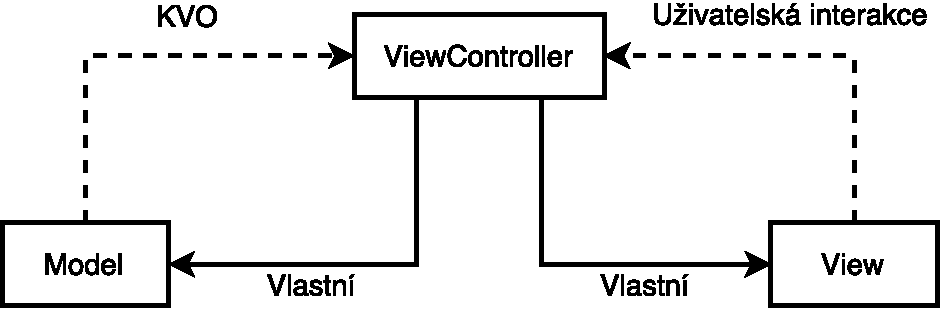
\includegraphics[width=0.75\textwidth]{assets/analysis-mvc-architecture.pdf}
	\caption{Architektura MVC}\label{fig:architektura-mvc}
\end{figure}

\begin{description}
  \item[Model] Reprezentuje perzistentní objekty, které aplikace využívá pro vnitřní logiku a prezentaci dat uživateli.
  Každý modelový objekt může být v relaci s libovolným počtem jiných modelových objektů.
  Tato vrstva je často reprezentována databází, příkladem mohou být databáze CoreData, Realm nebo SQLite.
  Ukázka \ref{code:mvc-model} prezentuje možnou podobu modelového objektu.
  \swiftcode{code:mvc-model}{Modelový objekt v architektuře \acrshort{mvc}}{assets/code/mvc-model.swift}

  \item[View] Datový objekt viditelný uživatelem. \texttt{View} obsahuje logiku pro vykreslení a interakci s uživatelem.
  Přestože se \texttt{View} standardně používá pro zobrazení modelových objektů nebo jejich úpravu, jsou od sebe tyto vrstvy striktně odstíněny.
  Na platformě iOS tuto vrstvu reprezentuje framework UIKit vytvořený Applem.
  Ukázkový kód \ref{code:mvc-view} zobrazuje možnou implementaci \texttt{View}.

  \item[Controller] Aplikační vrstva, která na základě vstupů z \texttt{View} aktualizuje a mění Model nebo překresluje \texttt{View} v případě, že zobrazovaná data už nejsou aktuální.
  Jedním z úkolů \texttt{Controlleru} je striktně zamezit přímé interakci mezi \texttt{View} a Modelem.
  Toto oddělení je zavedeno proto, aby \texttt{View} nemuselo znát konkrétní strukturu Modelu a aby Model nemusel obsahovat logiku formátování dat (cena, čas, ...) pro vykreslení.
  Dále se stará o navigaci mezi obrazovkami, síťování a interakci s uživatelem.
  Při rozdělení do obrazovek platí pravidlo, že jeden \texttt{Controller} obsluhuje jedno nebo více \texttt{View}.
  Ke korektnímu vykreslení \texttt{View} využívá libovoné množství modelových objektů.
  O jednu obrazovku se typicky stará právě jeden \texttt{Controller}, je ale možné jich použít více.
  Zjednodušenou implementaci lze vidět v ukázce \ref{code:mvc-view-controller}.
\end{description}

Z tohoto shrnutí vyplývá, že \texttt{Controller} je velmi blízce spjat s \texttt{View}. Toto propojení reprezentuje obrázek \ref{fig:massive-mvc}.

\subsubsection*{Modelový příklad použití}

Pro možné porovnání architektury jsem připravil scénář stažení libovolných dat na základě požadavku uživatele.
V \acrshort{mvc} by se architektura chovala takto:

\begin{itemize}
  \item Uživatel v aplikaci klikne na tlačítko \uv{Stáhnout data}.
  \item Tuto interakci odchytí \texttt{View} a upozorní \texttt{Controller}.
  \item \texttt{Controller} na základě upozornění stáhne data a předá je Modelu k uložení.
  \item Model ukládá data a notifikuje \texttt{Controller} o změně.
  \item \texttt{Controller} aktualizuje \texttt{View}.
  \item Nastane-li během stahování chyba, \texttt{Controller} vytváří nové \texttt{View} a chybu prezentuje uživateli.
\end{itemize}

\swiftcode{code:mvc-view}{View v architektuře \acrshort{mvc}}{assets/code/mvc-view.swift}

\subsubsection*{Shrnutí}

Shrneme-li vlastnosti vrstev, jejich klíčové role jsou:

\begin{itemize}
  \item Model udává, jakým způsobem jsou data uložena,
  \item \texttt{View} se stará o správné vykreslení předformátovaných dat,
  \item \texttt{Controller} se stará o ostatní logiku.
\end{itemize}

\swiftcode{code:mvc-view-controller}{ViewController v architektuře \acrshort{mvc}}{assets/code/mvc-view-controller.swift}

Pro zmíněné notifikace nabízí Apple řešení pomocí Delegate pattern návrhový vzor.
Tento návrhový vzor udává, že \texttt{Controller} musí naimplementovat specifické rozhraní, čímž se stane delegátem.
Jako delegát se pak může zaregistrovat na notifikace obejktů, jejichž rozhraní implementoval.

\acrshort{mvc} je v době psaní této práce nejpoužívanější architekturou a to především díky své jednoduchosti.
Při tvorbě větších aplikací ale nemusí být vhodné.
\texttt{Controller} se při nestandradním grafickém návrhu může stát velmi složitým, což výrazně snižuje jeho čitelnost a testovatelnost.
Z tohoto důvodu se \acrshort{mvc} často přezdívá \uv{Massive \texttt{View} Controller}.
Kvůli přímému napojení \texttt{Controlleru} na \texttt{View} se při testování jeho chování (behavior testing) musí využít simulátoru mobilního operačního systému.
Pro simulátor je navíc nutné naskriptovat uživatelův průchod aplikací, aby bylo možné testy automatizovat.

To zvyšuje časovou náročnost testování, dokonce v některých případech znemožňuje testování úplně (\texttt{Controlleru} nezle podvrhnout mock objekty).
Tento problém se snaží řešit architektura \acrfull{mvvm} od společnosti Microsoft.

\begin{figure}\centering
	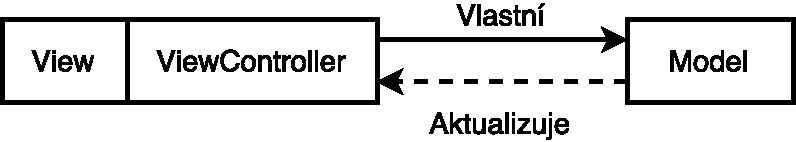
\includegraphics[width=0.75\textwidth]{assets/analysis-massive-view-controller.pdf}
	\caption[Role Controlleru v MVC]{Controller spjatý s View}\label{fig:massive-mvc}
\end{figure}

\subsection{MVVM: Model-View-ViewModel}\label{analyza-mvvm}

Z důvodu nárustu nároků na mobilní aplikace se v posledních letech rozmáhá architektura \acrshort{mvvm}.
Tato architektura vychází ze zmíněného \acrshort{mvc} a jejím základním úkolem je zjednodušit \texttt{Controller}.

\subsubsection*{Popis architektury} \label{architektura-mvvm-popis}

Za účelem zjednodušení \texttt{Controlleru} se ke stávajícím třem vrstvám přidává \texttt{ViewModel}, který se stará o přípravu dat z Modelu pro zobrazení a také o perzistenci změn.

\begin{description}
  \item[ViewModel] je objekt vlastněný \texttt{Controllerem} za pomoci kompozice.
  Pro \texttt{Controller} připravuje naformátované výstupy a poskytuje mu rozhraní pro vstupy.
  Výstupem se rozumí veškerá data, která jsou potřebná pro sestavení \texttt{View}.
  To může být např. datum ve specifickém formátu, cena včetně měny nebo informace o tom, kolik řádků bude obsahovat tabulka na obrazovce.
  Oproti \acrshort{mvc} tedy perzistentní data nejsou viditelná \texttt{Controlleru}, ale pouze \texttt{ViewModelu}.
  Ten je nejdříve připraví pro zobrazení.
  Vstupem může být libovolná interakce uživatele:
  změna textu v textovém poli, stisknutí tlačítka, ale i fyzický pohyb telefonem (otočení obrazovky).
  Na základě vstupů spouští \texttt{ViewModel} svou vnitřní logiku a generuje výstupy.
  Jednoduchou implementaci \texttt{ViewModelu} bez použití vstupů lze vidět v ukázce \ref{code:mvvm-view-model}.
\end{description}

\swiftcode{code:mvvm-view-model}{ViewModel v architektuře \acrshort{mvvm}}{assets/code/mvvm-view-model.swift}

Zodpovědnost \texttt{Controlleru} se zavedením \texttt{ViewModelu} dramaticky snižuje.
V ideálním případě je \texttt{Controller} zodpovědný pouze za správné sestavení \texttt{View} a napojení zfromátovaných výstupů na něj.
Dále pak za odchycení uživatelských interakcí a jejich propagaci do \texttt{ViewModelu}.
Toto chování zachycuje obrázek \ref{architektura-mvvm}.

\begin{figure}\centering
	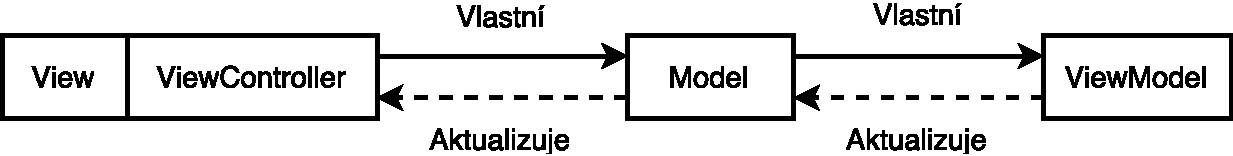
\includegraphics[width=0.9\textwidth]{assets/analysis-mvvm-architecture.pdf}
	\caption[Architektura \acrshort{mvvm}]{Architektura \acrshort{mvvm}}\label{architektura-mvvm}
\end{figure}

\subsubsection*{Modelový příklad použití} \label{architektura-mvvm-priklad}

Pro porovnání architektury s \acrshort{mvc} lze opět využít scénář pro stažení dat.
Pro tento scénář by se architektura \acrshort{mvvm} chovala následovně:
\begin{itemize}
  \item \texttt{Controller} napojuje výstupy \texttt{ViewModelu} na \texttt{View} a vytváří pravidla pro převod uživatelské interakce na vstupy \texttt{ViewModelu}.
  \item Uživatel v aplikaci klikne na tlačítko \uv{Stáhnout data}.
  \item \texttt{View} upozorňuje \texttt{Controller} na interakci uživatele, ten automaticky vytváří vstup pro \texttt{ViewModel}.
  \item \texttt{ViewModel} na základě vstupu stahuje data a předává je Modelu.
  \item Model po uložení notifikuje \texttt{ViewModel}, ten vytváří výstup pro \texttt{Controller}, který nechává překreslit \texttt{View}.
  \item V případě chyby vytvoří \texttt{ViewModel} chybový výstup, ten se pomocí \texttt{Controlleru} propaguje do \texttt{View}.
\end{itemize}

\subsubsection*{Shrnutí} \label{architektura-mvvm-shrnuti}

Vrstvy mají následující klíčové vlastnosti:
\begin{itemize}
  \item Model definuje jakým způsobem jsou data uložena a při změně notifikuje \texttt{ViewModel},
  \item \texttt{View} vykresluje na obrazovku naformátované výstupy a upozorňuje \texttt{Controller} při interakci uživatele,
  \item \texttt{Controller} sestavuje hierarchii \texttt{View}, napojuje zformátované výstupy \texttt{ViewModelu} na \texttt{View} a z uživatelské interakce vytváří vstupy pro \texttt{ViewModel},
  \item \texttt{ViewModel} načítá data Modelu. Na základě vstupů z \texttt{Controlleru} nebo změny Modelu generuje výstupy pro \texttt{Controller}.
\end{itemize}

Oproti \acrshort{mvc} je na tomto příkladu vidět snížení zodpovědnosti \texttt{Controlleru}.
Tato zodpovědnost se přesunula do \texttt{ViewModelu} (viz. ukázka \ref{code:mvvm-view-controller}).
Na první pohled nemusí být tato změna opodstatněná, protože logika aplikace nezmizela, jen se přesunula.
Právě to ale umožnilo (nebo minimálně zjednodušilo) způsob, jakým lze logiku testovat.
\texttt{ViewModel} generuje výstupy na základě vstupů, v testech tedy lze uživatelskou interakci podvrhnout a testovat pouze výstupy (není potřeba vytvářet \texttt{View} ani \texttt{Controller}).
Dodatečně lze otestovat i uživatelské rozhraní.
Protože logika aplikace je otestována pomocí testů \texttt{ViewModelu}, uživatelské rozhraní už stačí otestovat např. shodou \texttt{View} s referenčním obrázkem.

\swiftcode{code:mvvm-view-controller}{Controller v architektuře \acrshort{mvvm}}{assets/code/mvvm-view-controller.swift}

Při pohledu na notifikace je vidět, že přibyl typ, který nebyl v \acrshort{mvc} potřeba.
Jedná se o notifikace směrem z \texttt{ViewModelu} ke \texttt{Controlleru} (\texttt{ViewModel} nemá referenci na \texttt{Controller}, nemůže ho notifikovat přímo).
Některé výstupy \texttt{ViewModelu} je tedy potřeba sledovat v čase a na jejich změny reagovat.
Toto lze vyřešit pomocí \acrfull{kvo}, které nabízí Apple mezi standardními knihovnami.
\acrshort{kvo} umožňuje objektu zaregistrovat se na notifikace o změně stavu nějakého libovolného jiného objektu.
V případě \texttt{Controlleru} by se registroval na změny stavu výstupů \texttt{ViewModelu}.
Kdykoliv by se výstup změnil, \texttt{Controller} by dostal notifikaci.
Tento přístup ale není běžný pro použití s jazykem Swift.
Tento postup navíc neřeší synchronizaci vláken, z tohoto důvodu by mohlo docházet k nekonzistenci dat či neočekávanému chování.
Místo \acrshort{kvo} se nyní standardně používají reaktivní rozšíření, které popisuji v následujících kapitolách.

Přestože mnou implementovaná aplikace není v ohledu na uživatelské scénáře nijak složitá, obsahuje mnoho obrazovek.
Obrazovky jsou vysoce interaktivní a více se k jejich implementaci hodí reaktivní přístup.


\section{Synchronizace vláken aplikace} \label{analyza-synchronizace-vlaken}

Mobilní aplikace se svou povahou značně liší od běžných webových nebo desktopových aplikací.
Oproti zmíněným jsou často mnohem interaktivnější, tedy ovládané nejen běžnými vstupy, ale i vlastnostmi zařízení (GPS poloha, orientace zařízení, dostupnost periferií).
Aby tyto vstupy nekazily uživatelský zážitek, jsou v systému implementovány asynchronně.

Jako příklad lze vzít získávání polohy z družic.
To provádí telefon na vlákně v pozadí.
Tím je zaručené, že hlavní vlákno aplikace (které se mimo jiné stará o vykreslování) není blokované a s aplikací lze bez problému intereagovat.
Jakmile jsou dostupné informace o poloze, aplikace zažádá systém o prostředky na hlavním vlákně a získanou polohu prezentuje uživateli.

Tento přístup je v SDK poskytovaným Applem velmi obvyklý a využívá ho mnoho standardních knihoven.
Ne vždy je ale běžné, aby výsledek byl prezentovaný na hlavním vlákně.
Takový princip je využit u síťových požadavků.

Síťový požadavek se vykonává na vlákně v pozadí a na stejném vlákně je zpracována i odpověď ze vzdáleného serveru.
Je-li potřeba odpověď zpracovat na hlavním vlákně, musí vývojář explicitně čas na hlavním vlákně vyžádat pomocí Grand Central Dispatch či vlákna synchronizovat jiným spůsobem.
Od verze systému iOS 9 je navíc nemožné udělat síťový požadavek synchronně (blokovat vlákno, které požadavek vytvořilo až do konce zpracování) \cite{apple-whats-new-in-ios}.

Otázkou tedy zůstává jak správně synchronizovat všechny vlákna, která potřebují zpracovat data na hlavním vlákně.

Při analýze tohoto problému jsem se zaměřil na tři možná řešení.
První dvě jsou implementovány přímo v dodávaném SDK, třetí možnost je knihovna od společnosti GitHub.

\subsection{Grand Central Dispatch}

Grand Central Dispatch (zkráceně GCD) je technologie vyvinutá společností Apple přinášející optimalizovanou podporu pro aplikace fungující na vícejádrových procesorech.
GCD je implementována nad standardními systémovými vlákny, vývojáři ale nabízí mnohem jednoduší rozhranní.

Pro zjednodušení je využit princip front (z angl. queue), které jsou reprenzentovány třídou \textit{DispatchQueue}.
DispatchQueue je implementována jako \textit{thread-safe}, je tedy možné k nim přistupovat ve stejný okamžik z několik vláken najednou \cite{apple-concurrency-programming-guide}.
Do této fronty je možné vkládat jednotky práce, GCD se postará o to aby byly spuštěny na ve správném pořadí.
V závislosti na konfiguraci je pak umožňuje jednotlivé úkoly spouštět synchronně nebo asynchronně.

V základu je dostupná \textit{main} fronta, která je synchronní a umožňuje vykonat práci na hlavním vlákně.
Pro synchronizaci vláken stačí požadované jednotky práce přidávat do správných front  \ref{code:create-dispatch-queue}.

Je-li potřeba vytvořit vlastní frontu (z důvodu uvolnění času na hlavním vlákně), stačí specifikovat název fronty a její prioritu.
Vytvoření nové fronty běžící v pozadí je vidět v ukázce \ref{code:create-dispatch-queue}.

\swiftcode{code:create-dispatch-queue}{GCD: Vytvoření vlastní fronty}{assets/code/create-dispatch-queue.swift}

Přidání do libovolné fronty..

\subsubsection*{Quality of Service}

Pro možnost rozlišení priorit front využívá Apple Quality of Service (zkráceně QoS).
Díky QoS je možné určit, jakou prioritu bude mít danná fronta při rozdělování vláken.
V současné době existují čtyři QoS priority \cite{apple-prioritize-work-with-qos}:

\begin{description}
  \item[User-interactive] Práce, se kterou uživatel přímo interaguje.
  Tato fronta má nejvyšší prioritu, nejčastěji se v ní provádí překreslování uživatelského rozhranní či animace.
  Jednotlivé úkoly z fronty jsou vykonané ihned.
  \item[User-initiated] Práce, kterou zadal uživatel a vyžaduje okamžitý výsledek.
  Nejčastěji se stará o akce, které nastanou po interakci s některým z ovládacích prvků (např. tlačítko).
  \item[Utility] Práce, která vyžaduje více času pro své dokončení.
  Typicky se jedná o síťové požadavky nebo načítání dat.
  \item[Background] Práce s nízkou prioritou, kterou si nevyžádal uživatel.
  Využívá se zejména pro dávkové mazání souborů, synchronizaci nebo indexování databáze.
\end{description}

Při vytváření front je důležité správně volit prioritu.
Budou-li všechny fronty využívat jednu prioritu, může se stát, že systémová vlákna nebudou správně využita.
To by vedlo ke snížení výkonu aplikace a špatné uživatelské zkušenosti.

Přestože GCD je velmi zajímavá abstrakce nad standardními vlákny, jedná se stále o nízkoúrovňové API.
Mezi jednotkami práce nelze vyvářet závislosti či je řetězit.
Tuto možnost ale nábízí \textit{Foundation} framework pomocí \textit{NSOperationQueue}.

\subsection{NSOperationQueue a NSOperation}

NSOperationQueue a NSOperation je abstrakce nad metodou GCD zmíněnou víše.
Toto API je od verze systému iOS 4 implementováno právě pomocí GCD, nabízí ale nové možnosti přístupu k prováděným jednotkám práce.
Hlavním rozdílem oproti GCD je vyloučení pojmu \textit{vlákno}.
Jednotky práce nejsou nadále reprezentovány pomocí \textit{first class funkcí}, ale nově pomocí instancí tříd \textit{NSOperation} o jejichž správu se stará \textit{NSOperationQueue}. \cite{cocoacasts-nsoperation-vs-gcd}

\subsubsection*{NSOperation}

Pro reprezentaci jednotek práce se standardní funkce v GCD nejevily jako dostatečné.
S představením NSOperationQueue, je ale nově možné nad opakovanými jednotkami abstrakci pomocí tříd.
Toho lze docílit pomocí vytváření vlastních tříd dědících od NSOperation.

NSOperation představuje samostatnou jednotku práce (operaci).
Jedná se o abstraktní třídu zajišťující \textit{thread-safe} přístup ke správě stavu, priority a závislostí.

Jako úkol lze chápat například jednotlivé síťové požadavdy, zpracování vstupů a uživatele a jejich perzistence nebo komplexní výpočty.
Úkolem je možné označit ale i libovolnou strukturovanou jednotku práce, u které je potřeba udržovat stav nebo zpracovat její datový výstup.

Oproti CGD má objektový přístup výhodu nejen v přehlednější strukturování, ale i v možnosti vytváření závislostí a správě stavu \cite{apple-operation-queues}.

\begin{description}
  \item[Závislosti] definují, jaké další operace musí být vykonány před tím, než bude daná operace spuštěna.
  Přidat lze libovolný počet dalších operací, tím lze dosáhnout komplexního procesu za pomoci skládání menších bloků.
  Jako příklad lze uvést síťovou komunikaci, kde každý požadavek závisí na ověření dostupnosti internetu (první operace) a na patřičném ověření uživatele (druhá operace).
  Ke každému požadavku následně stačí přiřadit tyto dvě operace jako závislost, tím je zaručené že požadavek se pošle jen když je dostupné připojení k internetu a zároveň je uživatel ověřený.
  \item[Správa stavu] umožňuje operaci pozastavit, spustit znovu nebo zrušit.
  Oproti GCD, kde úkol, který se začal zpracovávat už nebylo možné zastavit, lze například do ovládání operací zapojit uživatele.
\end{description}

\subsubsection*{NSOperationQueue}

Obdobně jako GCD, je i zde potřeba určit kde a kdy se bude práce vykonávat.
Pro tento účel slouží fronta NSOperationQueue.
Tato fronta je implementována jako prioritní.
Tedy v momentě kdy je vložena operace s vyšší prioritou, bude vykonána dříve než stávající operace s nízkou prioritou (pokud to její závislosti dovolí).
Z tohoto odůvodu není zaručeno kdy se jednotlivé operace spustí.

Základní vytvoření operace a vložení do fronty je vidět na ukázce \ref{code:operation-queue-demonstration}.

\swiftcode{code:operation-queue-demonstration}{NSOperationQueue: Vytvoření fronty s operacemi}{assets/code/operation-queue-demonstration.swift}

\subsubsection*{Prioritizace úkolů}

Z důvodu potřeby prioritizace některých úloh je možné jedntlivým operacím nastavit prioritu.
V takovém případě se vždy jako první vykonají operace s vyšší prioritou, následně se přistupuje k těm s nižším.

\subsubsection*{Quality of Service}

Jednou z nejsilněších stránek NSOperationQueue je abstrakce front nad vlákny (tedy celého GCD).
V nastavení fronty lze zvolit stejně jako u GCD výchozí QoS.
Všechny operace pak budou vyžívat právě tuto prioritu.
Oproti GCD má však NSOperationQueue výhodu, že nepracuje pouze s jednou frontou.

To dává vývojáři možnost definovat QoS pro každou operaci zvlášť a to bez nutnosti vytvořát více front.
V závisloti na této vlastnosti je dále možné definovat, kolik operací může být \textit{maximálně} spuštěno v jeden okamžik.

\subsection{Reaktivní programování}\label{vlakna-rac}

Reaktivní programování získává poslední dobou velký zájem vývojářů \cite{oneagency-rx}.
Jedná se o programování založené na reakci na uživatelské vstupy.
Nejčastěji je tento princip spojován s prograváním uživatelského rozhraní, protože je implementováno asynchronně a neblokuje tedy hlavní vlákno aplikace.

Myšlenka reaktivního programování je nepřistupovat k datům jako stálým hodnotám, ale jako proudu (streamu) hodnot v konkrétní čas.
Implementací existuje více, např. Promise \cite{slaks-promise}, Callback \cite{yld-callback} či funkcionálně reaktivní programování.
V analýze jsem zabýval pouze funkcionálně reaktivním programováním, konkrétně imlementací v knihovně \textit{ReactiveCocoa}.




\chapter{Implementace}\label{implementace}

V této kapitole se budu podrobně věnovat použitým technologiím a implementaci jednotlivých funkcionalit.
V první části shrnu jaké technologie analyzované v kapitole \ref{analyza} jsem zvolil.
V dalších částech se věnuji konkrétním funkcionalitám navrženým podle analýzy API v kapitole \ref{analyza-api}.

\section{Použité technologie}

V této části se postupně zabývám jednotlivými body analýzy a rozebírám jaké řešení z těch, která jsem analyzoval, jsem zvolil pro implementaci.
Jedním z hlavních kritérií při konečném rozhodování byla slučitelnost jednotlivých částí.
Vzhledem k rozsahu implementace jsem si musel být jistý, že jednotlivé části budou fungovat správně v celé aplikaci.
Rozhodujícím faktorem tedy nebyla popularita jednotlivých řešení ale spíše jejich flexibilita.

\subsection{Architektura aplikace}\label{technologie-architektura}

Nejdůležitějším rozhodnutím bylo správné vybrání architektury.
Špatný výběr architektury by mohl mít dopad na celkovou funkčnost aplikace či znemožnit implementaci některých z vyžadovaných funkcí.

Po podrobném analyzování obou zmíněných architektur jsem se rozhodl využít \acrshort{mvvm}.
Přestože \acrshort{mvvm} není v současné době tak rozšířené, nabízí spoustu vlastností, které standardní \acrshort{mvc} nemá.

Silným argumentem je testování.
V architektuře \acrshort{mvvm} lze jednotlivé části otestovat samostatně.
K otestování logiky aplikace navíc není potřeba vizuální vrstva aplikace.

Neméně podstatným argumentem je čitelnost kódu.
Vrstva Controller obsahuje mnohem méně kódu a lze se v něm snáze orientovat.
ViewModel naopak neobsahuje žádné prvky uživatelského rozhraní a znázorňuje tak pouze způsob, jakým se daná část aplikace chová.
Jednotlivé vrstvy jsou od sebe striktně odděleny a dodržují princip jedné odpovědnosti \cite{toptal-srp}.

\subsubsection*{Implementace ViewModelu}

V části \ref{analyza-mvvm} kde jsem analyzoval architekturu \acrshort{mvvm} jsem naznačil strategii implementace.
ViewModel jsem se rozhodl implementovat jako logiku Controlleru, která jako rozhraní nabízí pouze vstupy či výstupy.

Vstupem označuji uživatelskou interakci, na základě které je potřeba vyžádat nová data nebo zobrazit jinou obrazovku.
Výstupem jsou zobrazovaná data, která jsou ViewModelem předformátovaná aby je Controller mohl přímo zobrazit pomocí View vrstvy.
Jiným výstupem pak může být informace o stavu dat či o jejich počtu (počet položek v seznamu).

Každá obrazovka vlastní svůj ViewModel.
Pro ten jsou dostupné tři protokoly: \textit{ViewModelInputs}, \textit{ViewModelOutputs} a \textit{ViewModelType}.
Tyto prokoly jsou konkrétně pojmenovány podle obrazovky, stejně tak ViewModel samotný a také Controller.
Definice rozhraní je vidět v ukázce \ref{code:viewmodel}.

\swiftcode{code:viewmodel}{Rozhraní objektu ViewModel}{assets/code/viewmodel.swift}

První protokol popisuje množinu vstupů, druhý množinu výstupů a třetí popisuje rozhraní ViewModelu.
Tím jsem dosáhl možnosti zaměňovat ViewModel obrazovky či sdílet jeden ViewModel mezi více obrazovkami.
Návrhem tohoto rozhraní jsem inspiroval v open source aplikaci Kickstarter, dostupné na portálu GitHub \cite{github-kickstarter}.

\subsubsection*{Implementace Controlleru}

Controller při inicializaci vyžaduje instanci ViewModelu.
Veškerou logiku obrazovky pak na ViewModel během svého životního cyklu deleguje.

Uživatelské vstupy jsou implementovány pomocí funkcí.
Controller sleduje uživatelskou interakci a volá patřičné funkce ViewModelu.
Výstupy z ViewModelu jsou pomocí UI bindings napojeny na View v metodě \textit{bindViewModel}, která je volána těsně po načtení View vrstvy do paměti.

Controller vyžaduje v konstruktoru instanci implementující protokol vstupů a výstupů, nikoli konkrétní třídu.

\subsubsection*{Coordinator}

\acrshort{mvvm} standardně nepoužívá objekt spravující navigaci v aplikaci.
Implementoval jsem proto další objekt nazvaný Coordinator.
Jedná se o objekt, který se stará o průběh jedné konkrétní části aplikace (flow).
Jakmile uživatel vyžaduje přechod na obrazovku mimo rozsah stávajícího Coordinatoru, vytvoří se nový Coordinator starající se o novou obrazovku a její životní cyklus.
Coordinator má také na starosti vytvoření ViewModelu a předání jeho instance Controlleru.

Scénář obrazovky se spustí metodou \textit{start}.
Po ukončení (uživatel chce zavřít obrazovku) volá Coordinator metodu \textit{completed} kde se uvolní naalokované zdroje.

S Coordinatorem spolupracuje ViewModel metodou delegate pattern.

\subsection{Synchronizace vláken}

Pro synchronizaci vláken jsem se rozhodl použít knihovny ReactiveCocoa a ReactiveSwift, tedy reaktivní přístup.
Díky těmto knihovnám lze jednoduše tvořit závislosti asynchronních operací.

S využitím knihovny ReactiveCocoa od verze 5.0 lze navíc využít tkzv. \textit{UI bindings}.
Ty zaručují, že hodnoty signálů jsou vždy zpracovány na hlavním vlákně a to i v momentě, kdy jsou odeslány z vlákna v pozadí.
ReactiveSwift pak zaručuje konzistenci dat mezi vlákny.
Dohromady tak tyto knihovny zamezují vzniku \textit{race condition} za běhu aplikace.
Více o těchto knihovnách lze zjistit z oficiální dokumentace \cite{github-reactiveswift} a \cite{github-reactivecocoa}.

Neméně podstatným faktorem byla i velmi dobrá integrace v architektuře \acrshort{mvvm}.
Pomocí operátorů nad signály lze formátovat vlastnosti modelových objektů (přidání jednotek, standardizace čísel, zástupné texty).
Takto naformátované signály zaručí, že kdykoliv se aktualizuje modelový objekt, jeho vlastnosti budou správně naformátovány.
ViewController tak vždy dostane data ve správném formátu bez ohledu na to, jakým způsobem byly změny na Modelu aplikovány.

\subsection{Síťová vrstva}

Síťovou vrstvu jsem se zpočátku rozhodl implementovat knihovnou Alamofire.
Důvodem byla snazší implementace a integrace do aplikace.
Protože nemá Alamofire striktně danou strukturu koncových bodů, bylo jednoduché implementovat dynamickou URL tiskárny.

Chybějící podpora reaktivního programování ale velmi brzy negativně zasáhla běh aplikace.
K synchronizaci vláken jsem nemohl využít ReactiveSwift a aplikace byla zatížena množstvím chyb vznikajících při vykonávání síťových požadavků a následné serializaci dat.

Z tohoto důvodu jsem se rozhodl využít knihovny Moya, která nabízí reaktivní rozšíření a je kompatibilní s ReactiveSwift.

Veškeré síťové požadavky nakonec využívají knihovnu Moya, s jejíž implementací chyby s vlákny vymizely.

\subsubsection*{Implementace Provider objektu}

Při implementaci jsem se neobešel se standardními objekty, které jsou běžné potřebné.
Provider objekt předimplementovaný v knihovně předpokládá, že adresa vzdáleného serveru je známá již během kompilace a neumožňuje ji zadat za běhu programu.
Z tohoto důvodu jsem také nemohl využít standardní definici koncových bodů pomocí TargetType protokolu, který URL vyžaduje staticky.

Rozhodl jsem vytvořit podtřídu \textit{DynamicProvider}, která v konstruktoru přijme URL serveru.
Místo využití protokolu TargetType jsem vytvořil nový protokol TargetPart, který má stejné rozhraní, jen nevyžaduje URL serveru.

Má implementace Provider objektu využívá tento nový protokol pro vytvoření požadavku.
Abych mohl využít třídu, od které můj objekt DynamicTarget dědí, musel jsem ještě vytvořit strukturu DynamicTarget, která implementuje rozhraní TargetType a využaduje tedy URL serveru.
Tu jí ale může poskytnout v konstruktutoru DynamicProvider spolu s TargetPart koncovým bodem.

Tím jsem dosáhl stejného rozhraní pro požadavky jako má nadtřída, jediným rozdílem je možnost dodat URL až při běhu aplikace.

\subsubsection*{Síťové požadavky mimo OctoPrint}

Pro umožnění zobrazení video streamu jsem opět potřeboval dynamickou URL, ale tentokrát pro každý požadavek (uživatel zadává pouze URL, nejsou žádné koncové body).
Tato implementace nebyla složitá, využil jsem standardních tříd knihovny Moya.
Vytvořil jsem nový objekt spravující koncové body a v něm definoval pouze jeden bod \textit{get}.
Ten pro zkonstruování využaduje koncovou URL a chová se tedy velmi podobně jako kdyby URL byla známá už v čase kompilace.

Při využití je ale nutné pro každý požadavek explicitně URL zadat.
To je krok který v DynamicProvider není nutný.

\subsection{Datová vrstva}

Jak vyplývá z části \ref{analyza-datova-vrstva} kde popisuji datovou vrstvu, rozhodl jsem se využít knihovnu Realm.
Díky jejím reaktivním rozšířením se skvěle hodí nejen k architektuře, ale i k síťové vrstvě.

Při implementaci jsem dospěl k závěru, že standardní cestou využití Realmu opakuji spoustu kódu.
Vytvořil jsem proto rozšíření pro ReactiveCocoa a její Cold signál.

Pro SignalProducer, který jako hodnotu nese Realm objekt jsem přidal dvě metody.
První z nich, \textit{fetch(collectionOf:)} umožňuje z databáze načíst kolekci.
Druhou metodou je \textit{fetch(classType:, forPrimaryKey:)}.
Ta vybere z databáze prvek podle primárního klíče.
Využití metod je vidět v ukázce \ref{code:realm-extensions}.

\swiftcode{code:realm-extensions}{Reaktivní rozšíření pro Realm}{assets/code/realm-extensions.swift}

Díky těmto rozšířením jsem odstranil spoustu duplicitního kódu, navíc jsem sjednotil rozhraní využívaných knihoven.
Mohl jsem díky tomu synchronizovat vlákna síťových volání a datové vrstvy pomocí ReactiveCocoa.

\subsection{Grafické prvky}

Pro ilustrace a ikony v aplikaci jsem se rozhodl využít framework Iconic.
Oproti zmíněnému Assets catalog v mém řešení výkon aplikace nezhoršuje, naopak poskytuje velmi snadným způsobem desítky ikon v jediném fontovém souboru.

Jako grafický font jsem vybral FontAwesome verze 4.7 \cite{fontawesome-web}.
Grafický font jsem využil pro ikony záložek na obrazovce detailu tiskárny ale také pro ikony, které nejsou běžně v systému dostupné.

Protože pomocí grafického fontu není možné vytvořit ikonu aplikaci, využil jsem také Assets catalog.
Využit je ale právě pro ikonu aplikace, ostatní potřebné ilustrace poskytuje Iconic.

Iconic v současné době není podporován správcem závislostí, který jsem si zvolil.
Z tohoto důvodu jsem potřebné soubory pomocí frameworku vygeneroval zvlášť a následně je do projektu vložil.

Současně jsem také nabídl autorovi frameworku pomoc s podporou pro jiné cesty distribuce.
Během implementace této práce se nám ale nepodařilo možnosti distribuce rozšířit.
Více informací o tomto tématu je dostupné na stránce projektu \cite{github-iconic-brew}.

\subsection{Správa závislostí}

Při výběru správce závislostí jsem své nároky směřoval především na ovlivnění kompilace aplikace.
V konečném důsledku pracují oba zanalyzované nástroje podobně, mají ale rozdílný přístup k linkování knihoven.

Přestože nastavení CocoaPods je mnohem snazší, z mého pozorování vyplynulo, že negativně ovlivňuje čas kompilace.
To je způsobeno častou kompilací jednotlivých knihoven a to i v případě, že jejich zdrojový kód nebyl upraven.
Dále jsem vypozoroval, že prostředí Xcode je s CocoaPods méně stabilní, přestává fungovat našeptávání a zvýrazňování syntaxe.

Z těchto důvodů jsem zvolil Carthage.
Počáteční nastavení bylo nepatrně složitější z důvodu ručního integrování knihoven do projektu.
Integrují se ale předem zkompilované knihovny, čas jednotlivých buildů aplikace se tedy nezvyšuje.
Linkování zkompilovaných knihoven má pravděpodobně za následek lepší integraci s Xcode.
Za dobu psaní práce se stalo jen výjimečně, že by se Xcode nečekaně ukončil.
Zlepšilo se také zvýrazňování syntaxe.
To fungovalo během psaní celé práce bez problému.

Výměnou za zlepšené fungování při lokálním vývoji byly problémy při kompilaci na CI serveru.
Nekompatibilita zkompilovaných knihoven s verzí Swift jazyka použitým při vývoji aplikace způsobila, že více než dvě třetiny kompilací na serveru selhalo.
Přehled jednotlivých buildů je vidět na \cite{travis-octophone-builds}.


\section{Seznam dostupných tiskáren}

Aplikace jsem navrhl tak, aby klíčové funkcionality byly dostupné s co nejkratším průchodem aplikace.
Jako úvodní obrazovku jsem zvolil seznam tiskáren.
V případě, že již uživatel aplikace dříve používal, zobrazí se v seznamu na prvních místech tiskárny, které si uživatel uložil.
Na dalších místech jsou pak tiskárny dostupné na stejné síti, které aplikace automaticky nalezla.

Pokud aplikace požadovanou tiskárnu nenalezla, je ze seznamu tiskáren možné přejít na obrazovku pro manuální přidání tiskárny.

\subsection{Implementace seznamu}

Abych dosáhl uživatelského rozhraní kompatibilního se zařízeními iPhone i iPad, rozhodl jsem se seznam implementovat pomocí CollectionView.
Z analýzy vyplynulo, že velmi podobné seznamy budou dostupné na většině obrazovek.
Rozhodl jsem se tedy zavést novou třídu pokrývající společnou logiku a výchozí nastavení nazvanou BaseCollectionView.

Tato základní třída se stará o barevné sjednocení obrazovek, zobrazování chyb a nastavení View pro prázdné obrazovky.
Jednotlivé obrazovky pak využívají třídy dědící z BaseCollectionView.

\subsubsection*{Sekce seznamu}

Seznam tiskáren je rozdělen na dvě základní sekce.
Pomocí rozdělení do samostatných sekcí jsem dosáhl vytvoření nezávislých řádkových indexů pro každou sekci.
ViewModel pro Controller poskytuje počet řádků pro každou ze sekcí samostatně.
Při vytváření seznamu stačí tedy ověřit pro jakou sekci se záznam v seznamu vytváří a následně ViewModel požádat o data s konkrátním řádkovým indexem číslovaným od nuly.

V případě jedné sekce by bylo nutné vzájmně porovnávat aktuální číslo řádku s počtem uložených tiskáren a tiskáren nalezených.
To požaduje komplexní výpočet a dává prostor mmoha chybám.

\subsubsection*{Uložené tiskárny}

První sekce zobrazuje tiskárny načtené z lokální databáze.
Při sestavování seznamu si pomocí \textit{delegate pattern} CollectionView nejdříve vyžádá počet prvků pro tuto sekci.
Controller tedy využije výstup ViewModelu a vrátí hodnotu jeho proměnné nazvané \textit{storedPrintersCount}.
Implementace této metody je vidět v ukázce \ref{code:printer-list-number-of-rows}.

\swiftcode{code:printer-list-number-of-rows}{Konfigurace počtu tiskáren v seznamu}{assets/code/printer-list-number-of-rows.swift}

V momentě kdy CollectionView ví kolik prvků bude zobrazovat, začne vyžadovat jednotlivé položky seznamu.
K tomu je opět využit delegate pattern.
Pro správné dodržení MVVM architektury nesmí Controller využívat modelové objekty.
Pro každou buňku je tedy potřeba vytvořit ViewModel, který ji bude obsluhovat.
Controller si pro řádkový index vyžádá od svého ViewModelu nový ViewModel buňky a ten jí.
Buňka se následně sama z ViewModelu nakonfiguruje.
Vyžádání ViewModelu buňky zachycuje ukázka \ref{code:printer-list-cell-viewmodel}.

\swiftcode{code:printer-list-cell-viewmodel}{Vytváření buňky v seznamu}{assets/code/printer-list-cell-viewmodel.swift}

\subsubsection*{Síťové tiskárny}

Tato část názorně ukazuje sílu MVVM architektury.
Přesto, že logika stojící za vyhledáním síťových tiskáren není triviální, ViewController zůstává velmi krátký a dobře čitelný.

Z pohledu Controlleru totiž logika není podstatná, důležité jsou výstupy z ní.
ViewModel pro seznam tiskáren jsem proto navrh tak, aby poskytoval obdobné rozhraní jako poskytuje pro uložené tiskárny.

Pro zobrazení druhé sekce seznamu stačí CollectionView předat informaci o počtu síťových tiskáren a buňkám předat odpovídající ViewModely.
Toho se docílí ve stejných metodách jako pro uložnené tiskárny.
Počet síťových tiskáren je uložen v proměnné \textit{networkPrintersCount} a ViewModely je možné získat metodou \textit{networkPrinterCellViewModel}.

\subsection{Automatické aktualizace}

Abych zajistil přijemnou uživatelskou zkušenost z aplikace, rozhodl jsem se seznam tiskáren implementovat jako \textit{push-based}.
Tato strategie uvádí, že při změně dat jejich vlastník (např. ViewModel) upozorní své odběratele (Controller).
Každý odběratel se sám rozhodne, jakým způsobem informaci využít.
V mé konkrétní implementaci lze vidět rozdíl od \textit{pull-based} strategie v automatických aktualizacích.

Strategie \textit{pull-based} spočívá v tom, že data jsou dostupná na požádání.
To znamená, že změní-li se data (např. bude-li nalezena nová síťová tiskárna), odběratel si je explictině musí vyžádat.
Zde vzniká otázka, jak často se dotazovat, zda změna proběhala či nikoli.

Odpověď se odvíjí konkrétního využití.
Některé data není potřeba po načtení aktualizovat vůbec, jiná naopak prvidelně s krátkými intervaly.

\bigskip

Abych zajistil konzistenci napříč celou aplikací, rozhodl jsem se využít strategii push-based směrem z ViewModelu do Controlleru.
Controller sleduje signál změn a pokaždé když se na signálu objeví hodnota (obvykle typu Void), překreslí odpovídající View.

Za pomoci UI bindings frameworku ReactiveCocoa jsem napojil signál změn na metodu překreslení seznamu.
Controller tedy nemusí o data explicitně žádat, kdykoliv se totiž změní vyšle ViewModel signál a tabulka se překreslí.
Pro překreslení se využívá stejný postup jako při iniciálním načtení, nehrozí proto problém s čátečnou nekonzistencí.
Výsledkem je, že uživatel vidí na obrazovce vždy aktuální data.
Ukázka \ref{code:printer-list-ui-binding} demonstruje překreslení seznamu pomocí UI bingins.

\swiftcode{code:printer-list-ui-binding}{Překreslení CollectionView pomocí UI bindings}{assets/code/printer-list-ui-binding.swift}

\subsection{Přidání tiskárny}

V momentě kdy nebude požadavaná tiskárna automaticky nalezena a zároveň ji uživatel dříve nepřidal, je možné tiskárnu přidat ručně.
Přidání tiskárny se odehrává na nové obrazovce.
Na tu se uživatel dostane stisknutím tlačítka \uv{+} na obrazovce se seznamem tiskáren.

Pro vytvoření obrazovky je potřeba nový Controller a k němu odpovídající ViewModel.
Za zprostředkování nové obrazovky zodpovídá Coordinator zmíněný v sekci \ref{technologie-architektura}.

Controller seznamu tiskáren vytvoří vstup pro svůj ViewModel, ten na základě vstupu notifikuje Coordinator o uživatelské interakci.
Coordinator má předem definováno jakým způsobem na interakce reagovat.
Průběh je vidět v ukázce \ref{code:printer-list-coordinator-flow}.

Na základě notifikace Coordinator vytvoří potřebné objekty k sestavení obrazovky a ovrazovku prezentuje uživateli.
Až do ukončí tohoto flow je seznam tiskáren neaktivní.

Pokud uživatel tiskárnu úspěšně přidá, seznam je automaticky aktualizovaný díky push-based strategii.

\swiftcode{code:printer-list-coordinator-flow}{Průběh zobrazení nové obrazovky}{assets/code/printer-list-coordinator-flow.swift}


\section{Přidání nové tiskárny}

Obrazovka přidání tiskárny slouží pro případ, kdy uživatel chce ovládat novou tiskárnu a nenalezl ji v seznamu síťových tiskáren.
Pro úspěšné přidání tiskárny je nutné zadat její název, \acrshort{url} či IP adresu a přístupový token.
Volitelně je možné také přidat url adresu, na které se vyskytuje video stream z web kamery natáčející průběh tisku.

\subsection{Validace formuláře}

Jako u každé aplikace, která přijímá uživatelské vstupy i v mé implementaci je nutné ověřit platnost zadaných údajů.
Jelikož se jedná o logiku, je validace umístěna ve ViewModelu.
Text zadaný uživatelem se při každé změně odešle ViewModelu, který všechny vstupy zvaliduje.
Na základě platnosti kombinace vstupů vyšle ViewModel booleanovskou hodnotu Controlleru.
Controller pomocí UI bindigs sváže tuto hodnotu s blokací tlačítka \uv{Přihlásit}. 

Je-li formulář platný, tlačítko je povolené.
V opačném případě je zablokované a nelze stisknutím spustit jeho interakci.

Hodnoty formuláře jsou validované pomocí operací nad signály.
Signály vstupů jsou nejprve zkombinovány a následně map operátorem převedeny na booleanovskou hodnotu.
Použití validace nad signály je vidět v ukázce \ref{code:add-printer-validation}.

\swiftcode{code:add-printer-validation}{Validace formuláře pomocí signálů}{assets/code/add-printer-validation.swift}

\subsection{Uložení tiskárny}

Ve chvíli kdy je formulář ověřený, může uživatel připojení uložit do lokální databáze.
Uložení provede pomocí tlačítka \uv{Připojit}.
ViewModel upozorněný na interakci uživatele načte aktuální hodnoty formuláře a vytvoří požadavek na tiskárnu.

Je-li odpověd od tiskárny pozitivní (status kód odpovědi je v rozmezí 200 až 299), pak se hodnoty uloží do lokální databáze.
Coordinator je následně upozorněn na ukončení scénáře a obrazovku zavře.
Díky reaktivnímu přístupu a push-based strategii se rovnou tiskárna zobrazí v seznamu mezi dostupnými k použití.
ViewModel ani ViewController seznamu nemusí být o výsledku přidání tiskárny nijak notifikovány, o propagaci této informace se postará datová vrstva aplikace.

V případě selhání požadavku je vytvořena chybová hláška.
Díky reaktivním rozšířením, které jsem vytvořil pro ViewController třídu chybu zobrazit pomocí UI bindings.

Ukázka \ref{code:add-printer-login-request} zjednodušeně implementuje vytvoření požadavku a následné zpracování odpovědi od tiskárny.

\swiftcode{code:add-printer-login-request}{Vytvoření požadavku pro přihlášení k tiskárně}{assets/code/add-printer-login-request.swift}



\section{Ovládání tiskové hlavy}

Při implementaci ovládání jsem se inspiroval rozhraním OctoPrint, které je znázorněno na obrázku \ref{fig:octoprint-controls}.
Pohyb hlavy je možný po všech osách.
Aby bylo uživatelské rozhraní intuitivní, sjednotil jsem osy $x$ a $y$ do ovladače pro jednu ruku a osu $z$ do ovladače pro druhou.

\image{fig:octoprint-controls}{Ovládání tiskové hlavy v prostředí OctoPrint}{assets/implementation-octoprint-controls.png}

Rozhraní je tvořeno pomocí tlačítek, kde každá osa má jedno tlačítko pro pohyb v kladném a jedno pro pohyb v záporném směru.
Dále každý z ovladačů obsahuje tlačítko \uv{Domů}, které zavede tiskovou hlavu na souřadnici 0 v patřičných osách.

\subsection{Pohyb hlavy}

Jelikož jsou prvky tvořeny tlačítky, je pohyb implementovaný pomocí požadavků pro každou interakci zvlášť.
\texttt{Controller} pro každý stisk vytvoří vstup \texttt{ViewModelu}, ten následně vytváří požadavky na tiskárnu.

Požadavek pro posun hlavy je implementovaný genericky parametrizovaný množinou os a směrem.
Aby UI nebylo zbytečně komplikované, rozhodl jsem uživateli neumožnit explicitně zvolit o jakou vzdálenost se má hlava posunout.
Každý požadavek tedy posune hlavu po dané ose o 10 mm vpřed nebo vzad.

Každý uživatelský vstup je namapovaný na právě jeden vstup \texttt{ViewModelu}.
Tím jsem dosáhl jednoduchého rozhraní \texttt{ViewModelu} a odstranil potřebu využití složitých řídících konstrukcí (switch konstrukce či řetězené podmínky).
Implementace je znázorněna v ukázce \ref{code:printer-controls-request}.

\swiftcode{code:printer-controls-request}{Implementace pohybu tiskové hlavy}{assets/code/printer-controls-request.swift}

\subsection{Ovládání trysky}

Z důvodu možnosti čištění trysky jsem přidal na tuto obrazovku tlačítko pro manuální tavení filamentu.
Obdobně jako u pohybu tiskové hlavy ani zde jsem neumožnil uživateli zvolit množství.
Při uživatelské interakci (stisku tlačítka \uv{Tavit}) aplikace vždy nechá roztavit 5 mm.

Implementace tohoto požadavku se velmi blízce podobá požadavkům na pohyb tiskové hlavy.


\chapter{Testování}\label{testovani}

\todo{Aktualizovat kapitolu o testech}

\todo{Využití dockeru}

V kapitole o testování se podrobněji zabývám způsoby a postupy naznačenými v kapitolách \ref{analyza-mvvm} a \ref{vlakna-rac} o architektuře \acrshort{mvvm} a reaktivní programování.

Testováním software se rozumí postupy a procesy, pomocí kterých lze měřit, zda testovaný software (či jeho části) splňuje požadované nároky či nikoliv.
Opakovaným aplikováním těchto postupů lze v softwaru nalézt chyby, nedostatky nebo chybějící vlastnosti oproti dodané specifikaci.
Výsledky testování následně vypovídají o kvalitě softwaru a o míře splnění specifikace. \cite{software-testing-definition}

\bigskip

V této práci jsem využil dva typů testů.
Jako první techniku jsem zvolil testování chování (z anglického \texttt{behavior tests}).
Ty ověřují zda aplikace na sadu vstupů vrací odpovídající výstupy.

Další technikou jsou testy uživatelského rozhraní.
Pomocí nich lze ověřit, zda během vývoje nových funkcionalit nedošlo k poškození stávajícího uživatelského rozhraní.
V následujícím shrnutí se těmto technikám věnuji podrobněji.

\section{Testy chování}\label{testovani-bdd}

Chování jednotlivých modulů aplikace se testuje pomocí zkoumání plnění svých závazků.
Testované objekty mají definované své rozhraní a závisloti, tím jsou deklarovány i závazky objektu, které musí splnit.
Závazky určují, jakým způsobem by měl objekt působit na zbylé části aplikace a jaké schopnosti a funkce má.
Ze schopností a funkcí lze odvodit jakým způsobem se má objekt chovat.
Testovaným objektem může být libovolný modul aplikace.
Složitost a rozsah testů se odvíjí od počtu závazků objektu.
Testování probíhá tak, že vlastnosti objektu jsou pomocí rozhraní měněny a sleduje se, jestli se objekt na základě změn chová podle očekávání. \cite{objcio-bdd}

V reálném světě si lze jako objekt představit auto.
Jako změnu vlastnosti můžeme lze použít vyčerpání nádrže.
Očekávaným chováním auta následně je, že přestane být pojízdné a rozsvítí kontrolku řidiči.
Auto projde testem chování, právě když při prázdné nádrži je nepojízdné a svítí kontrolka.

Tento princip testování využívám pro testování View Modelu a Modelu (viz. kapitola MVVM: Model-View-ViewModel).
Díky otestování dostatečného rozsahu logiky aplikace, lze usuzovat, že v produkčním nasazení se vyskytne jen nepatrné množství chyb.
View vrstvu následně není samostatně nutné testovat, protože z testů View Modelu je jisté, že data jsou správně připravena k zobrazení.
Testy pomocí porovnání skutečného vzhledu s očekávaným (zmíněno v testech uživatelského rozhraní) jsou tedy dostačující.

Obdobně jako testy rozhraní i tyto testy se pouštějí při vývoji až několikrát denně.
Slouží také jako dobrý ukazatel kvality aplikace a dokáží určit její rozsah.

S pojmem \textit{testování chování} je velmi blízce spjat \textit{vývoj řízený testováním chování} (z anglického Behavior Driven Development, zkráceně BDD).
V tomto přístupu k vývoji se před konkrétní implementací nejdříve nadefinuje, jakým způsobem se mají testované komponenty chovat.
Následně se sestavují testy, které vyžadují úplné implementování vyžadovaného chování.
Tím má objekt definované, jaké rozhraní musí implementovat a jaké závislosti bude vyžadovat.
Testy jsou popisovány takzvaným DSL.
To je jazyk který pomocí kombinace klíčových slov a textového popisu definuje jak se komponenta má v určitou chvíli chovat.
Ukázka \ref{code:bdd-dsl} znázorňuje DSL v testovacím frameworku Quick.
Jakmile jsou vytvořené testy, přechází se k implementaci.
Při implementování se vybere test, kterým má aplikace projít a implementuje se pouze takový kód, který zaručí průchod tímto testem.
Takto se postupuje, dokud objekt neprojde všemi testy. \cite{objcio-bdd}

\swiftcode{code:bdd-dsl}{Použití DSL pro definici testu}{assets/code/bdd-dsl.swift}


\section{Testy uživatelského rozhraní}\label{testovani-ui}

\todo{Přepsat, přidat informace o snapshot testech}

Testování uživatelského rozhraní si klade za cíl ověřit správné sestavení komponent grafického rozhraní.
Pomocí interakce s komponentami se také zkoumá, jakým způsobem komponenty reagují.
Na rozdíl od testů chování přistupují tyto testy k aplikaci jako k celku a zacházejí s ní obdobně jako by s ní zacházel uživatel. Tyto testy tedy nemají přístup k vnitřní implementaci aplikace.
Jelikož nevyžadují během chodu zásah člověka (test \textit{nahrazuje} jeho přítomnost), mohou být pouštěny automaticky.
Standardně se tedy pouští při implementaci každé nové funkce, mnohdy až několikrát denně. \cite{apple-ui-testing}

Protože tyto testy z jsou v mém případě pouze nadstavbou nad \textit{testy chování} vysvětlené níže, rozhodl jsem se je implementovat pomocí referenčních obrázků.
Testy tedy pro každý podstatný krok scénáře obsahují referenční obrázek, jak by obrazovka měla v danou chvíli vypadat.
Pokud se vzhled s referenčním obrázkem shoduje, test projde.
Nevýhodou tohoto přístupu je nutnost přegenerování referenčních obrázků v momentě, kdy se vzhled obrazovky (úmyslně) změní byť o jediný obrazový bod.
Podstatnou výhodou tohoto přístupu je ale nezávislost na implementaci.
Pokud se implementace změní, s velkou pravděpodobností to výsledky testů neovlivní.

\section{Průběžná integrace}

Průběžná integrace (z anglického \textit{Continous integration}, zkráceně \texttt{CI}) je praktika vývoje software, při které členové týmu integrují svou práci mnohdy až několikrát denně.
Každá integrace je automaticky ověřena kompilací na buildovacím serveru a spuštěním testů.
Tato technika si klade za cíl odhalid integrační chyby aplikace co nejdříve je to možné. \cite{gitlab-use-ci}
To má za následek snížení časové náročnosti implemetace nových funkcí bez rizika narušení funkcionalit původní aplikace.

Nové funckionality se běžně skládají z nového kódu, upraveného produkčního kódu a upravených testů.
V momentě kdy vývojář označí funkcionalitu za kompletní, odešle své změny na vzdálený buildovací server, kde se aplikace zkompiluje a otestuje.
Integrace je následně provedena jen v případě, že celý proces proběhl bez chyby.
Jak je zjevné, při této technice je zásadní vysoké pokrytí aplikace testy.

Průběžné integrování je často velmi blízce vázáno na správu zdrojových kódů.
Některé systémy jako GitHub či GitLab je dokonce možné nastavit tak, aby by změny byly přidány do hlavní větve až ve chvíli, kdy build projde bez komplikací. \cite{travis-ci-building-pr}

Pro průběžnou integraci je na trhu dostupných mnoho řešení.
Rozhodoval jsem se mezi použitím komerčních řešení Travis CI a Circle CI.
První zmíněná možnost se jeví v open-source komunitě velmi populární a dalo by se říct, že je pro \texttt{CI} téměř synonymem.
Podle nezávislého průzkumu z roku 2016 využívá Travis CI téměř pětinásobek uživatelů než ostatních poskytovatelů dohromady. \cite{oregonstate-ci-survey}

Druhé řešení jsem chtěl vyzkoušet kvůli rostoucí popularitě. \cite{circleci-popularity}
Bohužel je kompilace na operačním systému macOS pro open-source projekty možná až po individuálním schválení. \cite{circleci-pricing}
Z tohoto důvodu jsem nakonec zvolil první řešení, kde je kompilace na systému macOS pro studenty zdarma.

\subsection{Statická analýza kódu}

Spolu s roustoucím týmem a rostoucím zdrojovým kódem se často zavádí směrnice programování.
Tyto směrnice udávají jakým způsobem je kód formátovaný.
Při dodržování těchto směrnic se kód stává konzistentním a dobře čitelným, to má za následek zrychlení vývoje a zvyšuje udržitelnost kódu.
Aby nebylo nutné analyzovat kód ručně, existují nástroje které analýzu automatizují.

Pro zajištění konzistence jsem použil nástroj \texttt{SwiftLint} od společnosti \texttt{Realm}.
\texttt{SwiftLint} je nástroj obsahující sadu pravidel pro statickou analýzu kódu.
Mimo jiné kontroluje správné zarovnání kódu, délky řádků či názvy proměnných.
V době psaní práce obsahuje tento nástroj dohromady téměř osmdesát pravidel.
Ve své implemetaci jsem se rozhodl vynechat dvě pravidla, které jsem nepovažoval za stěžejní a jejich dodržování by z mého pohledu vedlo ke snížení čitelnosti.
Kromě těchto dvou pravidel jsem využil i možnost vypnout pravidla pro určité části kódu.
Nejčastěji se jednalo o pravidla na kontrolu délky metod.

Tuto analýzu zajišťuje buildovací server před začátkem kompilace.
Pokud nejsou v kódu závažné porušení směrnice, pokračuje se ke kompilaci.
V opačném případě nastane chyba a je nutné kód opravit a integraci pustit znovu.


\section{Průběžné doručování}

Průběžné doručování (z anglického \textit{Continuous delivery}, zkráceně \textit{CD}) je způsob, kterým lze nasadit nové funkcionality, změny konfigurace či opravy chyb do produkčního prostředí.
Cílem této praktiky je automatizovaně aplikovat opakované postupy potřebné k vydání aplikace.
Tím lze minimalizovat množství chyb, které by vývojář jinak mohl při vydávání způsobit.
Vývojáři stačí v tomto případě pouze doručování spusti, server zařídí aby aplikace byla správně nasazena.

Kromě minimalize výskytu chyb tato technika snižuje čas vývoje.
Díky automatizovanému vydávání mají vývojáři více času na samotný vývoj.
Tím lze zaručit vyšší kvalitu kódu, nižší náklady na vývoj a také častější aktualizace software. \cite{continuousdelivery-what-is-ci}

Přestože pro svou práci nemám reálné produkční prostředí, rozhodl jsem se \textit{CD} použít pro distribuci testovací verze aplikace.
Díky tomu jsem mohl jednotlivé verze vydávat v průběhu vývoje velmi rychle a ověřit funkčnost aplikace na skutečných zařízeních.
Vydání verze jsem nastavil na každé nahrání zdrojových kódů do repozitáře.
Po statické analýze a kompilaci byla aplikace nahrána do prostředí Fabric, odkud si ji mohli registrovaní testeři stáhnout.

\section{Lokální testování}

Protože aplikace komunikuje výhradně s tiskárnou, musí být tiskárna dostupná i během vývoje.
Abych nemusel tiskárnu pořizovat, využil jsem možnost vytvořit virtuální tiskárnu.

S využitím technologie Docker jsem vytvořil kontejner s nainstalovanou aplikací OctoPrint.
Pomocí konfiguračního souboru jsem povolil vytvoření virtuální tiskárny.

OctoPrint jsem takto mohl mít spuštěný lokálně na počítači.
Po připojení OctoPrint k virtuálnímu portu tiskárny jsem mohl vyvíjet aplikaci i bez nutnosti vlastnit tiskárnu.

V ukázce \ref{code:docker} demonstruji spuštění kontejneru s virtuální tiskárnou z příkazové řádky svého počítače.

\begin{listing}[htbp]
\caption{\label{code:docker}Spuštění virtuální tiskárny pomocí Docker}
\begin{minted}[linenos, bgcolor=bgcode]{bash}
docker run -p"3200:5000" josefdolezal/virtuprint-docker 
\end{minted}
\end{listing}


\begin{conclusion}
  Cílem práce bylo vypracování mobilní aplikace pro platformu iOS umožňující nastavovat 3D tiskárny a tisknout z nich.

Výsledná aplikace umožňuje zobrazit přehled aktuálního tisku, správu souborů a nastavení 3D tiskárny.
Pomocí aplikace je také možné sledovat video stream z webové kamery připojené k tiskárně.
Uživatel také může vybrat soubor ve svém zařízení, nahrát ho do tiskárny a následně vytisknout.

V aplikaci lze komunikovat s libovolnou tiskárnou dostupnou na místní síti, která je aplikací automaticky nalezena.
Uživatel může velmi jednoduše takto tiskárnu přidat a obsloužit celý tisk.

\bigskip

Během implementace jsem se snažil většinu pozornosti věnovat architektuře aplikace.
Mnoho částí jsem proto v průběmu implementace několikrát přepsal.

Velkou výzvou bylo implementovat aplikaci reaktivně.
S reaktivním programování jsem doposud neměl žádné zkušenosti.
Nyní jsem ale rád, že jsem se takto rozhodl.
Využití reaktivního přístupu mi ušetřilo mnoho práce a velmi pravděpodobně i mnoho chyb, které bych jinak standardní cestou do aplikace zanesl.

\bigskip

Jsem přesvědčený, že díky využití zvolené architektury jsem také zvýšil testovatelnost aplikace.
Přesto, že jsem testy aplikace nikdy dříve nepsal, nebylo složité je s toutou architekturou vytvořit.

\subsection*{Výhled do budoucna}

V budoucnu je možné do vývoje aplikace přizvat programátory pohybující se pravidelně v prostředí 3D tisku a rozšířit ji tak v komunitě.
Z tohoto důvodu jsou zdrojové kódy práce volně dostupné jako open source.
Aplikaci je díky tomu možné rozšířit o nové funkcionality v případě aktualizace API OctoPrint.

V současné době ale neplánuji aplikaci distrubuovat běžným uživatelům obchodem App Store.

\end{conclusion}

\bibliographystyle{csn690}
\bibliography{bibliography}

\appendix

\chapter{Seznam použitých zkratek}
% \printglossaries
% \begin{description}
%
% \end{description}

\chapter{Obsah přiloženého CD}

\begin{figure}
	\dirtree{%
		.1 readme.txt\DTcomment{stručný popis obsahu CD}.
		.1 exe\DTcomment{adresář se spustitelnou formou implementace}.
		.1 src.
		.2 impl\DTcomment{zdrojové kódy implementace}.
		.2 thesis\DTcomment{zdrojová forma práce ve formátu \LaTeX{}}.
		.1 text\DTcomment{text práce}.
		.2 thesis.pdf\DTcomment{text práce ve formátu PDF}.
		.2 thesis.ps\DTcomment{text práce ve formátu PS}.
	}
\end{figure}

\end{document}
